\documentclass[12pt,a4paper,oneside]{article}
% nagyon sok kép esetén meggyorsítható a fordítás a draft móddal
% \documentclass[12pt,a4paper,oneside,draft]{report}
% ekkor a képek nem renderelődnek ki, csak placeholder lesz mérethelyesen
\usepackage[utf8]{inputenc} % mindenképp maradjon az utf-8 kódolás
\usepackage[magyar]{babel}
\usepackage[T1]{fontenc}
\usepackage{amsmath}
\usepackage{amsfonts}
\usepackage{amssymb}
\usepackage{graphics} % grafikus elemek, képek berakásához
\usepackage{epsfig} % eps importáláshoz
\usepackage{listings}
\usepackage{sectsty}
\usepackage{enumerate}
\usepackage{lastpage}
\usepackage{setspace}
\usepackage{hyperref} % PDF hivatkozásokhoz kell
\usepackage[hang]{caption}
\usepackage{titling} % a title, author parancsok szabad használatához
\usepackage{pgfplots}
\usepackage{tikz}
\usepackage{subcaption}

% a TikZ rajzoló modul, és a kapcsolási rajz készítő modul, ha kell
%\usepackage{tikz}
%\usepackage{circuitikz}

% az A4 oldal margóinak és méreteinek beállítása
\usepackage[left=25mm,right=25mm,top=20mm,bottom=25mm]{geometry}\pagestyle{plain}

% A sorköz távolság beállítása
% egyszeres sorköz
\singlespacing
% 1,5 sorköz
% \onehalfspacing

% A hivatkozások, és linkek átállítása alapértelmezett színre, fekete-fehér nyomtatáshoz optimalizálva
\hypersetup
{
  	colorlinks,
  	citecolor=black,
 	linkcolor=black,
  	urlcolor=black
}

% --------- A hallgató által kitöltendő rész! --------- %

% a dolgozat típusa
\title{Mérési Jegyzőkönyv} 

% a dolgozat szerzője
\author{Kozma Dávid Márk}

% a dolgozat típusát adjuk meg tárgyesetben, kisbetűvel (pl.: diplomatervet, szakdolgozatot, témalabor beszámolót stb.)
\newcommand{\dokumentumtipus}{jegyzőkönyv} 

% a dolgozat témája
\newcommand{\dokumentumcim}{ADSB Radar csomag demodulálása}

% --------- A hallgató által kitöltendő rész! --------- %

\begin{document}
\begin{titlepage}

    \begin{figure}
    \centering
    
\includegraphics[width=100mm,keepaspectratio]{figures/logo/bme.pdf}
    \end{figure}
    
    \centering
    \textbf{Budapesti Műszaki és Gazdaságtudományi Egyetem}\\
    \textbf{Villamosmérnöki és Informatikai Kar}\\
    \textbf{Szélessávú Hírközlés és Villamosságtan Tanszék}\\
    \vspace{5mm}
    
\includegraphics[width=40mm,keepaspectratio]{figures/logo/hvt_logo_only_fixed_vector_inverted.png}  \\
    \vspace{47mm}
    \Huge
    \dokumentumcim\\
    \vspace{57mm}
    \Large
    \thetitle \\
    \vspace{10mm}
    \Large
    \textbf{\theauthor}\\
    \vspace{10mm}
    \the\year
    
    
    \end{titlepage}
\tableofcontents
\lstset{
  language=C,                % choose the language of the code
  numbers=left,                   % where to put the line-numbers
  stepnumber=1,                   % the step between two line-numbers.        
  numbersep=5pt,                  % how far the line-numbers are from the code
  backgroundcolor=\color{white},  % choose the background color. You must add \usepackage{color}
  showspaces=false,               % show spaces adding particular underscores
  showstringspaces=false,         % underline spaces within strings
  showtabs=false,                 % show tabs within strings adding particular underscores
  tabsize=2,                      % sets default tabsize to 2 spaces
  captionpos=b,                   % sets the caption-position to bottom
  breaklines=true,                % sets automatic line breaking
  breakatwhitespace=true,         % sets if automatic breaks should only happen at whitespace
  title=\lstname,                 % show the filename of files included with \lstinputlisting;
}

\section{Mérés célja}

A mérés célja a szoftverrádiók, szoftveres jelfeldolgozási technikák, valamint a kooperatív
módon működő szekunder radarok szabványos üzenetváltásának módjával való
megismerkedés.

\section{Mérés}

\subsection{Elsőfordítás}
\begin{figure}[h]
    \centering
    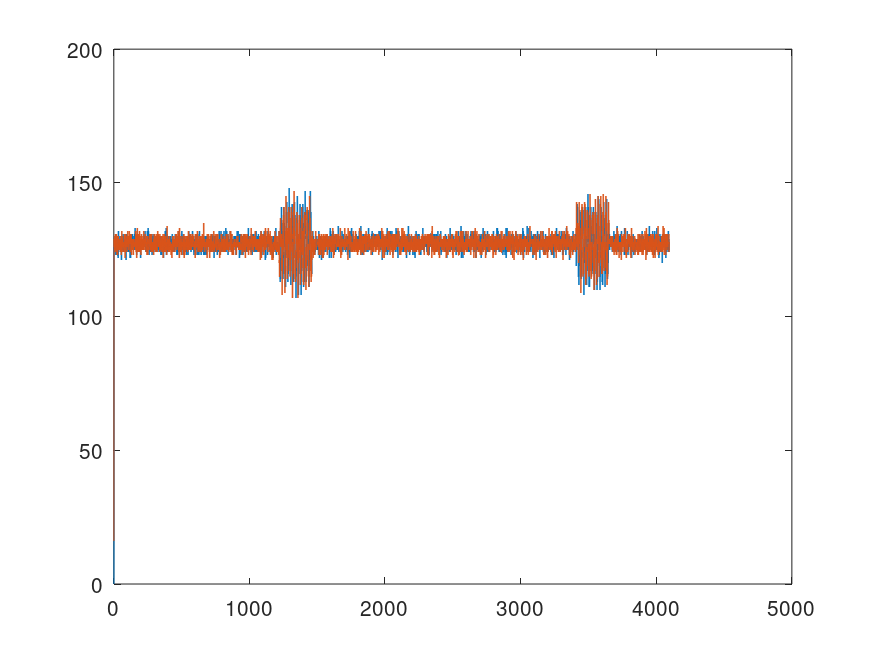
\includegraphics[width=0.9\textwidth]{../meres/result/elso_forditas.png}
    \caption{Első fordítás}
    \label{fig:first}
\end{figure}
\newpage
\subsection{Abszolút érték meghatározása}
\begin{lstlisting}
    abs_val=iq_to_abs[buffer[bix]][buffer[bix +1]];
\end{lstlisting}
\begin{figure}[h]
    \centering
    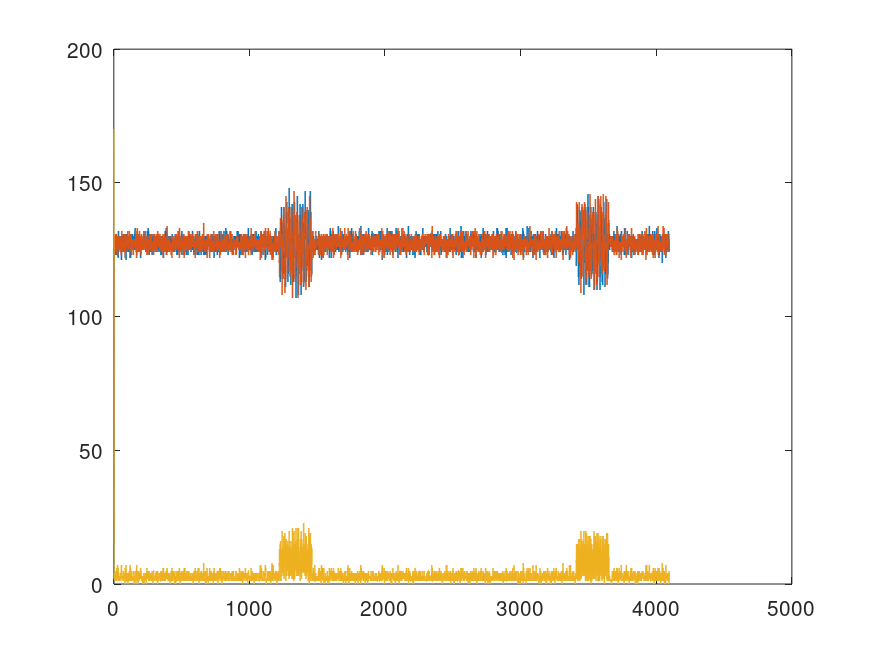
\includegraphics[width=0.9\textwidth]{../meres/result/abs_value.png}
    \caption{Abszolút érték meghatározása}
    \label{fig:abs}
\end{figure}

\newpage
\subsection{Döntési küszöb meghatározása}
\begin{lstlisting}
accumulator -= fifo[fptr];
accumulator += abs_val;
fifo[fptr] = abs_val;
i = (fptr+(FIR_LEN/2))%FIR_LEN; // The pointer calculation was wrong here.
fptr++;
fptr = fptr%FIR_LEN;
\end{lstlisting}
\begin{figure}[h]
    \centering
    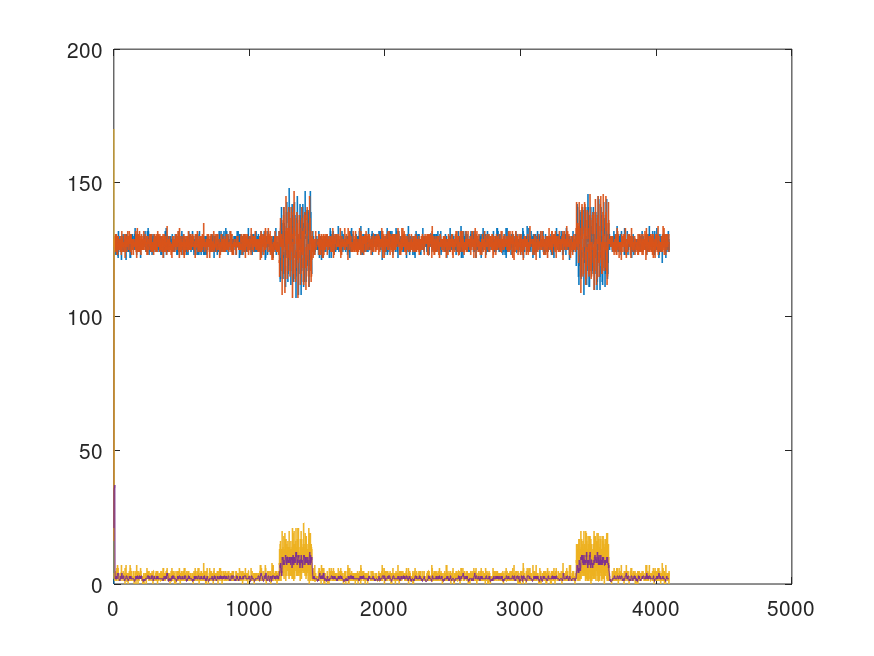
\includegraphics[width=0.9\textwidth]{../meres/result/dontes.png}
    \caption{Döntési küszöb meghatározása}
    \label{fig:deceison}
\end{figure}

\newpage
\subsection{Preamble detekció és csomag dekódolás}
\begin{lstlisting}
// Decoding
if (fifo[i] > (accumulator/FIR_LEN))
    bit = 1;
else
	bit = 0;
	// ADS-B packet search and print
	if (stm < 16)
	{
		if(bit == adsb_preamble[stm])
			stm++;
        else
			stm = 0;
    }
	else if((stm>=16)&&(stm<PCKT_LEN))
	{
		if (stm==16) printf("*");
		if ((stm%2)==0)
		{
			printf("%d",bit);
			hex=hex|bit;
			j++;
			if(j==8) {
                printf("%02x",hex);
				hex = 0;
				j = 0;
			}
			else hex = hex<<1;
		}
            stm++;
	}
	else
	{
		printf(";\r\n");
		stm = 0;
	}
\end{lstlisting}
\begin{figure}[h]
    \centering
    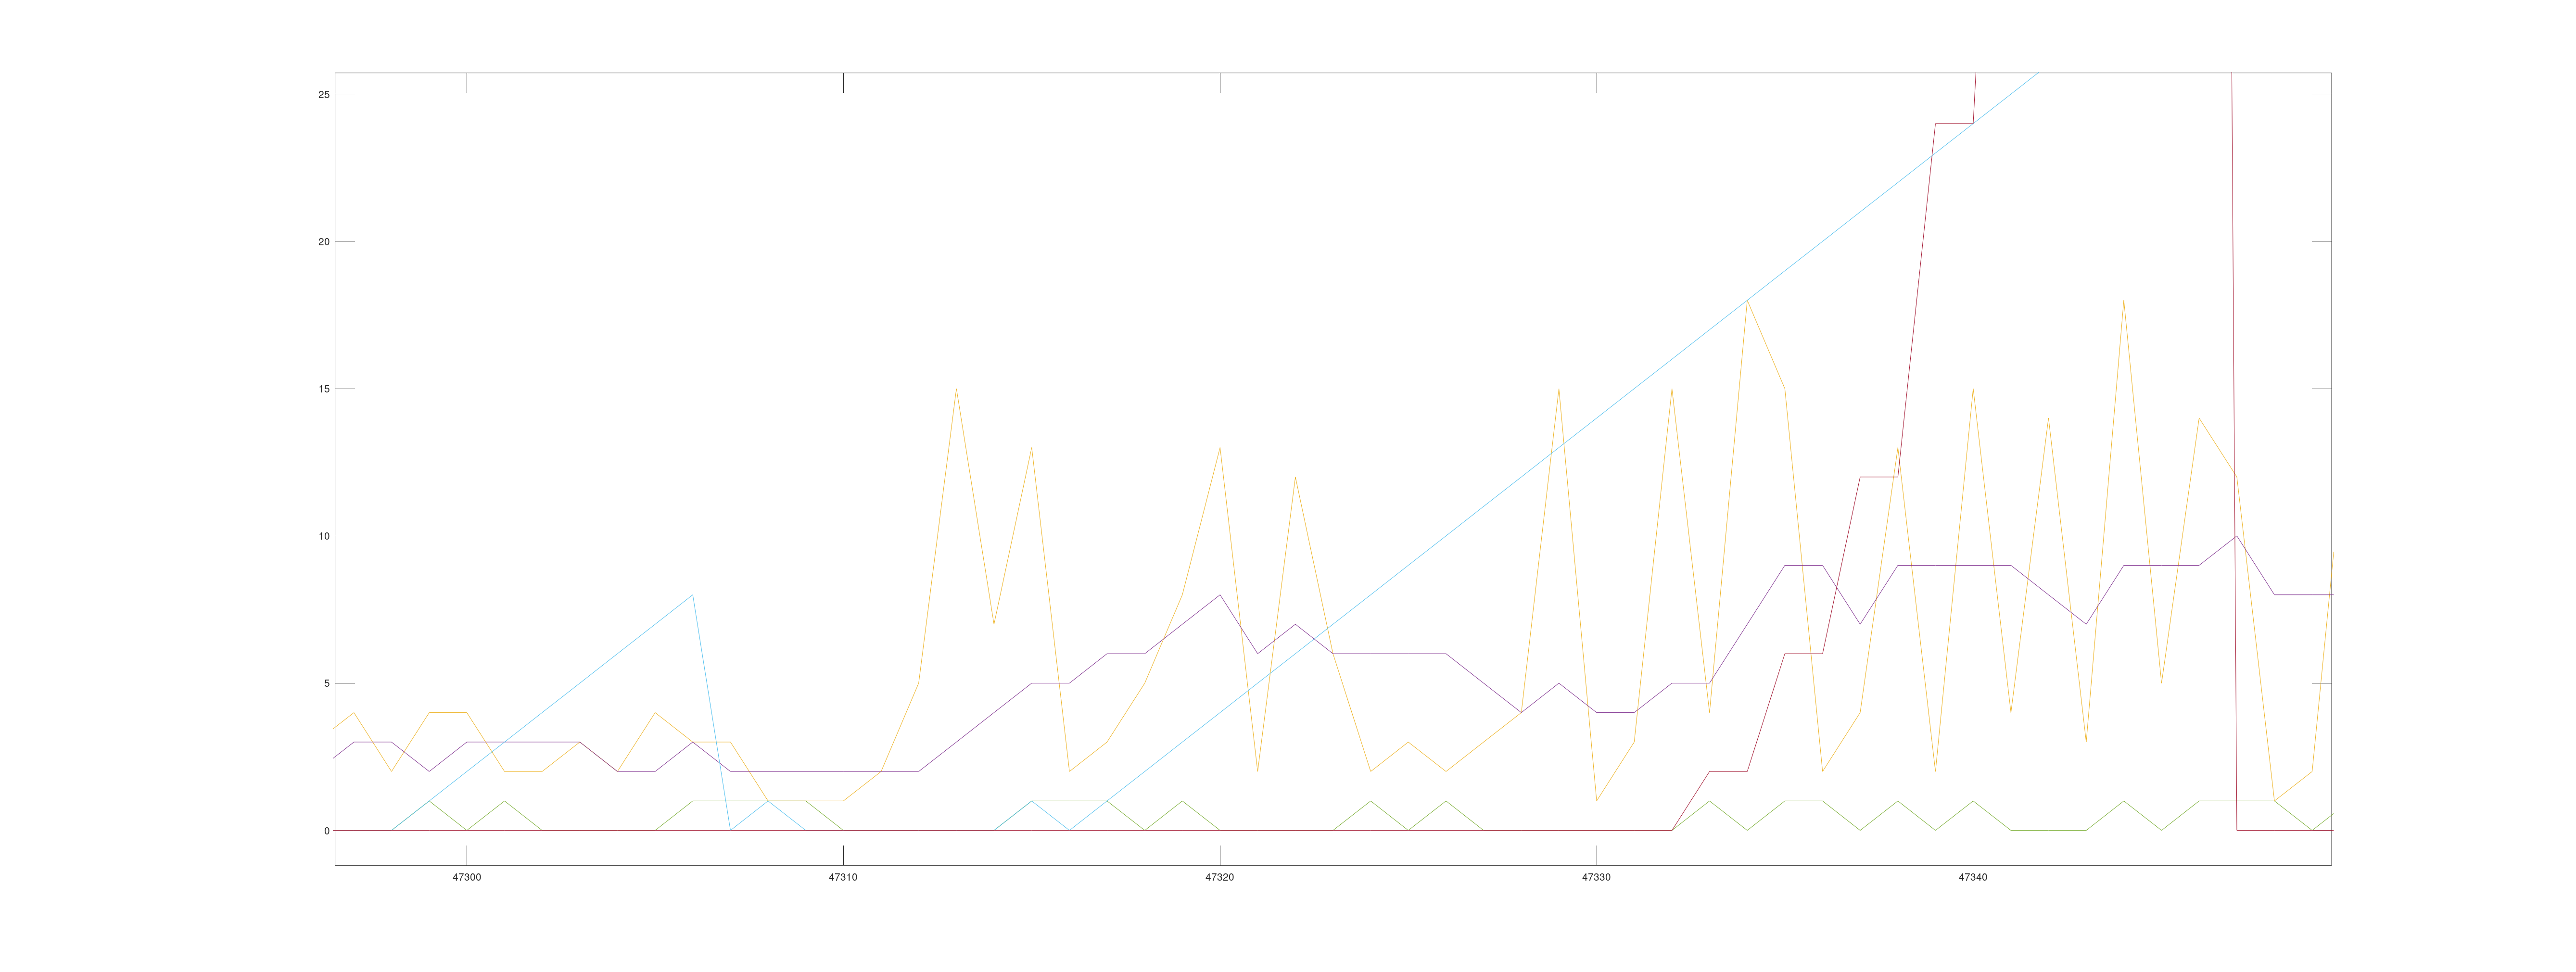
\includegraphics[width=1\textwidth]{../meres/result/preambledet_datacalc.png}
    \caption{Preamble detekció és csomag dekódolás}
    \label{fig:deceison}
\end{figure}

\newpage
\subsection{Dekódolt csomagok}
\begin{lstlisting}
    *27ae747474b5402ee534150216ec;
    *9047480610518315835820efe698;
    *9047480610518315835820efe698;
    *9047480610518315835820efe698;
    *9047480614518315835828cfe490;
    *4ed3d1a1cb9227d62e92a8649999;
    *91228288a45bd71164818c18dc84;
    *9047480690518115835820efe698;
    *90474a0690518315835820efe698;
    *9047480490518315835820efe698;
    *9047480692518315835820efe698;
    *9047480690518315a35820efe698;
    *90474a0610518315035820efe698;
    *9047480610518315835820efe698;
    *ad1a5535289b24084a1d443092c1;
    *9047480610518315a35820efe698;
    *9047480610518315835820efe698;
    *9047480614518315835820ebe698;
    *9046c80610518305a358206fe488;
    *9047480610518315835820ebe698;
    *7ec5ab848051793902592323ec32;
    *90474806105183158358206fe698;
    *9047480610518315835820efe698;
    *9447480610518315835820efe698;
    *9047480610118315a35820efe698;
    *9047480610518315835820efe698;
    *9047480610518315835820efe698;
    *9047480610518315835820efe698;
\end{lstlisting}

\newpage
\subsection{RTL SDR teszt}
Miután sikeresen megvalósítottam a dekódoló programot, a működést RTL SDR segítségével is tesztelltem.
\begin{lstlisting}
Using device 0: Generic RTL2832U OEM
Found Rafael Micro R820T tuner
Exact sample rate is: 2000000.052982 Hz
[R82XX] PLL not locked!
Sampling at 2000000 S/s.
Tuned to 1090000000 Hz.
Tuner gain set to automatic.
Reading samples in async mode...
Allocating 15 zero-copy buffers
*78c35a622544a031d20f70fa9c2c;
*511ccda8dd8ea921248d05cd8568;
*a5045b55eb51961349bcc4162351;
*9a15c14b5a9668ca0a42fcc9d089;
*f42e698aca6e52445bd3553a8a21;
*ea72e63cf94029a397dfe4553aaa;
*c55daf622dcb459609700a669b4a;
*208ab7304a1b3e3354b9c88eda8e;
*5d06a2e96991fd15006e57574894;
*28004b0dca73491b65286a5950d1;
*8f91826965ec68ba44931e4cfcc1;
*a8458b0dfffd3d376004f42a1c54;
*5586170fb4e8528366dd7ad28020;
*a7b5811eb3ae2955a2a24c145c62;
*a0001998e97a0b35a02541c756ce;
*b833542f9dd9ae8dcf893324fa07;
*a3d40cbaa450aa4b0962b64aeb8c;
*c480a724b0a9b24c1fddbb924c0d;
*8ab2d8e8575ade6fcebc73d126a3;
*a573365746ac34f04b906852cbba;
\end{lstlisting}

\subsection{Kiértékelés}
A mérés sikeresnek tekinthatő mert, a mérés során sikerült az adsb jelet demodulálni illetve a csomagokat is megfelelően dekódolni.\\
\\
A mérés forráskódja illetve a mérés során használt adat fájlok illetve a mérési eredmények a következő linken elérhetőek: \url{https://github.com/kozdavaa/adsb_meres}

\end{document}